%!TEX root = ../../csuthesis_main.tex
\chapter{系统功能实现与实验验证}

\section{系统整体运行流程}

本系统基于 Carla 仿真平台与 Python 接口开发,围绕视觉目标检测、跟踪与行为意图识别功能进行集成,形成一套具备实时性与可视化能力的自动驾驶感知子系统。该系统可在 Carla 环境中实现目标感知、意图推断与图形界面交互的完整闭环流程,为后续风险决策或辅助控制提供先验输入。

系统以 client\_bounding\_boxes.py 为主控脚本,其运行流程可分为以下几个关键步骤:

仿真环境初始化:程序首先通过 carla.Client 与 Carla 仿真服务建立连接,并加载预设的地图场景(如 Town10)。随后生成本车(ego vehicle)及环境交通流,配置摄像头等传感器并完成同步模式的启用。

实时图像获取与处理:车辆前置 RGB 摄像头不断采集画面帧图,系统利用 Carla 原生的投影功能从场景中提取每个车辆的 3D 边界框,并将其投影到图像平面,作为检测输入。

目标选择与跟踪处理:系统通过图像中心最近原则选择一个主目标作为跟踪对象,并以 DeepSORT 算法对其进行跨帧关联,保持稳定目标 ID。

行为意图识别:在跟踪信息基础上,结合目标速度、运动方向与中心点位移变化,利用物理建模方法对其进行行为趋势判定,输出“靠近”“远离”“危险靠近”等语义描述。

可视化与数据记录:系统将所有边界框、目标编号与意图分析文字实时绘制在主界面中,用户可通过键盘控制车辆行驶。同时,系统每隔若干帧自动将图像与标注信息保存为数据集,供后续训练与评估使用。

图像渲染部分采用 Pygame 实现,整合图像帧、边界框、速度信息、追踪 ID 和意图结果,统一绘制至显示窗口中,形成直观易读的运行界面。为了支持后续模型训练与效果回溯,系统还内置图像帧与标注信息的自动保存机制,每隔固定帧数将图像与对应 JSON 格式的边界框与速度数据写入本地数据集目录中。此外,系统还集成了模块级别的运行时间统计功能,在每帧处理结束后输出各阶段处理时长,并在运行一定帧数后将详细耗时记录导出为 CSV 表格,以便开展性能分析与优化研究。

通过上述流程的实现,本系统不仅在仿真环境下完成了从感知到理解再到预警的全流程闭环,还具备良好的可视化展示能力与运行稳定性,为后续章节中功能演示与性能评估奠定了坚实基础。

\section{界面展示}

系统基于 pygame 实现实时渲染窗口,在 Windows 系统上运行稳定,图像帧率维持在约 8~10 FPS。在主界面中,用户可清晰看到如下信息:

\textbf{•前视图图像帧:}显示本车前方道路环境、其他车辆等元素;

\textbf{•目标边界框:}每个检测到的车辆被标注为 3D 投影框;

\textbf{•跟踪目标编号:}被追踪目标在框上方显示 Tracked ID;

\textbf{•意图分析结果:}在跟踪目标框的上方显示当前系统判断的意图(如“危险靠近”、“目标远离中”等);

\textbf{•速度信息显示:}在边界框上标记目标当前速度(单位:m/s);

\textbf{•系统状态输出:}在终端控制台实时输出当前帧耗时、目标状态等信息,辅助调试与评估。

用户可使用键盘控制本车行为(如油门、制动、转向),以测试系统在不同驾驶状态下的感知鲁棒性。为了验证本系统在 Carla 仿真平台中的运行效果,本节通过一系列功能界面截图展示系统的关键功能模块与动态交互过程。系统运行过程中,各模块协同完成车辆环境感知、目标筛选、轨迹跟踪与行为意图判别,形成稳定的视觉处理与风险提示机制。

\begin{figure}[H]
    \centering
    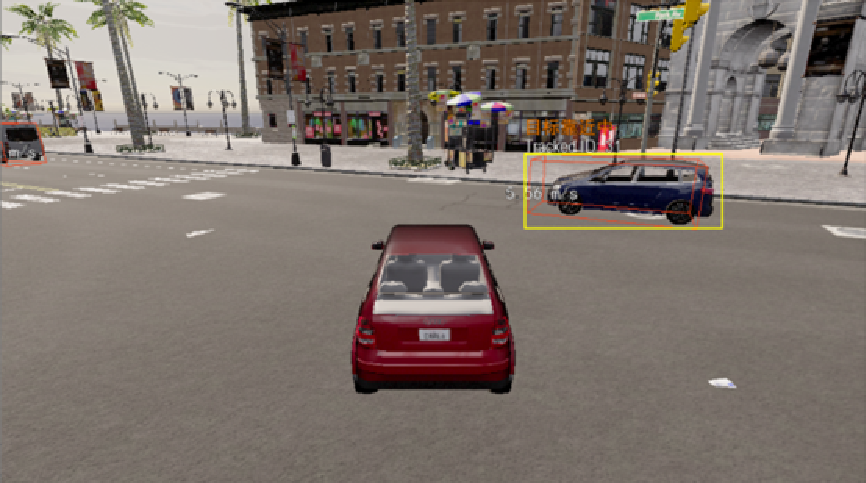
\includegraphics[width=0.8\textwidth]{images/图13 意图识别演示图(目标靠近).pdf}  % 引用转换后的 PDF 文件
    \caption{意图识别演示图(目标靠近)}
    \label{fig:example_image}  % 可用于引用此图片
\end{figure}

\begin{figure}[H]
    \centering
    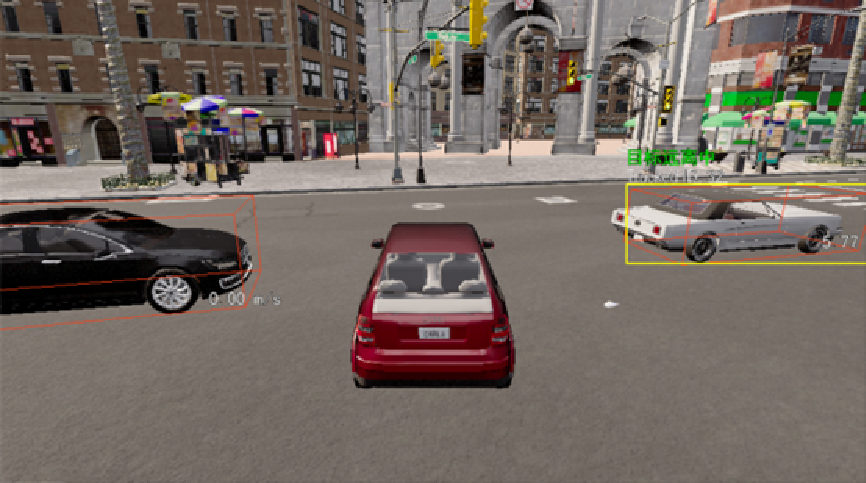
\includegraphics[width=0.8\textwidth]{images/图14 意图识别演示图(目标远离).pdf}  % 引用转换后的 PDF 文件
    \caption{意图识别演示图(目标远离)}
    \label{fig:example_image}  % 可用于引用此图片
\end{figure}

\begin{figure}[H]
    \centering
    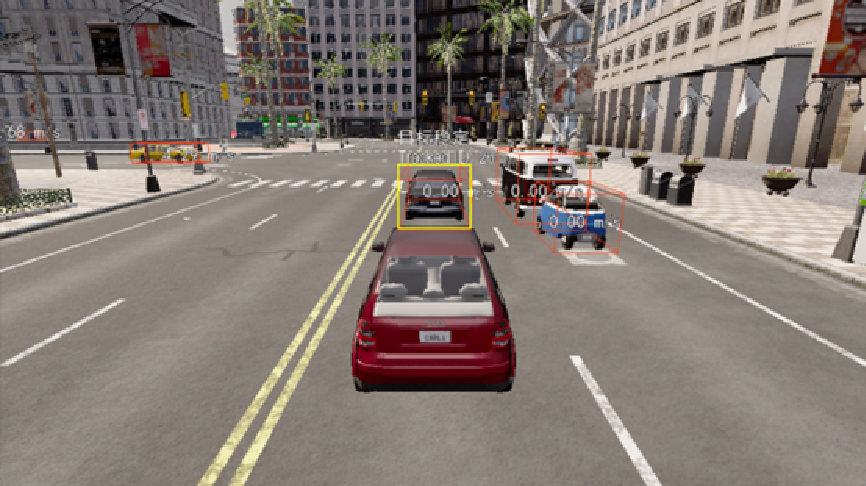
\includegraphics[width=0.8\textwidth]{images/图15 意图识别演示图(目标稳定).pdf}  % 引用转换后的 PDF 文件
    \caption{意图识别演示图(目标稳定)}
    \label{fig:example_image}  % 可用于引用此图片
\end{figure}

\section{用户交互与运行控制}

本系统设计过程中,充分考虑用户的交互体验与控制便捷性,通过键盘操作与实时图像反馈构建了较为完善的人机交互机制。系统主要依赖 Pygame 库实现交互接口,使用户可在仿真运行过程中随时控制车辆运动、调整观察角度并观察感知结果。

在车辆控制方面,用户通过键盘按键即可完成油门、制动、转向及手刹等基础驾驶行为。具体而言,按下 W 键实现车辆前进,S 键控制倒车,A/D 键分别用于左转与右转,Space 键则用于触发手刹功能。ESC 键可用于随时退出仿真运行,确保系统在用户终止时能够平稳释放资源,关闭所有传感器与窗口。系统在每帧循环中读取键盘输入并转换为 Carla 控制命令,从而实现对车辆的连续控制。

在感知交互方面,用户通过主界面可以直观地观察每一帧图像中感知与识别的结果。系统自动绘制车辆边界框,并在被跟踪目标的框体上方显示其 ID 号及行为意图判断结果。这些信息均实时更新,帮助用户理解系统当前感知状态与意图识别判断。在出现高风险情况(如危险靠近)时,系统通过红色高亮文字进行警示,从而增强用户的注意力,实现辅助驾驶提醒效果。

此外,系统还提供了自动数据采集与保存功能,支持在后台持续记录图像帧与标注信息,无需人工干预。该机制便于后续离线模型训练与性能评估,提升系统的可扩展性与工程价值。用户可通过配置参数设定数据采集频率和存储格式,以满足不同实验需求。

本系统在用户交互设计方面力求简洁明晰、操作灵活,配合 Carla 仿真平台稳定的底层支持,构建了一个具备真实驾驶控制体验与智能感知反馈能力的测试平台,能够有效支撑相关算法的开发验证工作。

\begin{figure}[H]
    \centering
    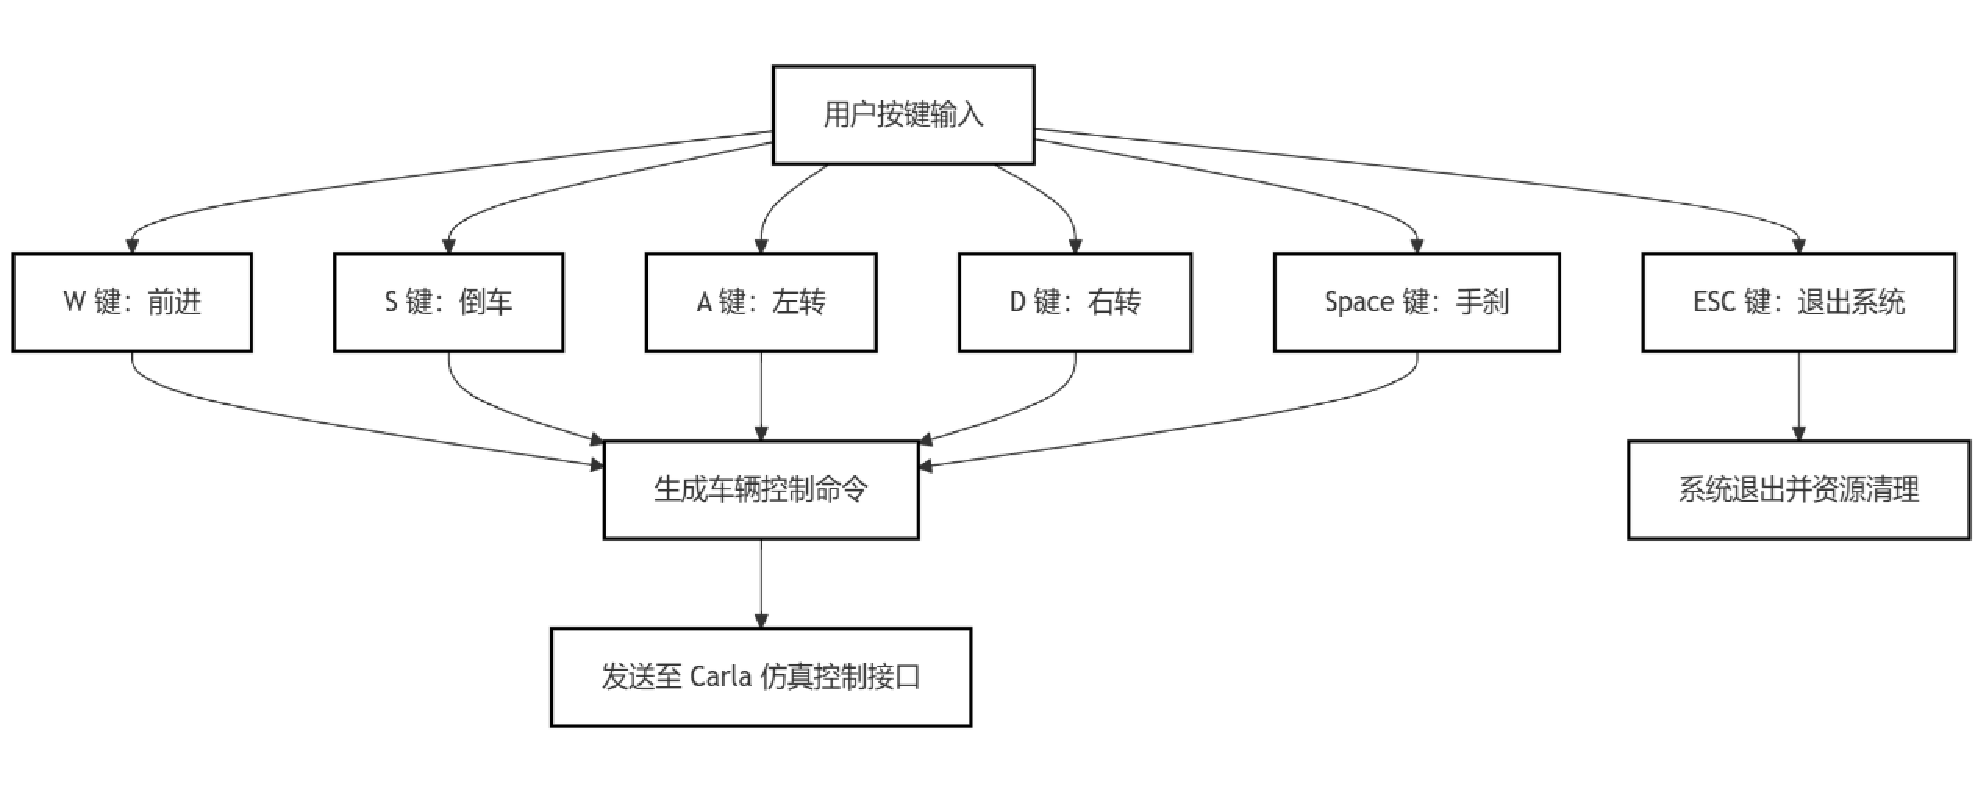
\includegraphics[width=0.8\textwidth]{images/图16 用户键盘控制映射关系示意图.pdf}  % 引用转换后的 PDF 文件
    \caption{用户键盘控制映射关系示意图}
    \label{fig:example_image}  % 可用于引用此图片
\end{figure}


\begin{tabular}{l l}
%  \verb|\songti| & {\songti 宋体} \\
%  \verb|\heiti| & {\heiti 黑体} \\
%   \verb|\kaiti| & {\kaiti 楷体}
\end{tabular}
